\documentclass{article}
\usepackage[T1]{fontenc}
\usepackage{lmodern}
\usepackage{graphicx}
\usepackage{amsmath,amssymb}
\usepackage[a4paper,margin=2cm]{geometry}
\usepackage[absolute,overlay]{textpos}
\setlength{\TPHorizModule}{1mm}
\setlength{\TPVertModule}{1mm}
\usepackage[indonesian]{babel}
\usepackage{hyperref}
\setlength{\emergencystretch}{2em}
% unit: Halaman 9

\begin{document}

% === Halaman 9 (python/native) ===

9

Plainteks:   otpadalahcipheryangtidakbisadipecahkan

Kunci:          trjkdndkdwerylgrgdkopcegyhbdwjbtrfhgvk

       Cipherteks: HKYKGNOKKYMGFPXPGQQHXFEQZPTDZRQXTFOQVX 

• Aturan enkripsi dan dekripsi yang digunakan persis sama seperti pada  Vigenere 

Cipher, bedanya tidak ada perulangan kunci secara periodik.

• Enkripsi: C = (P + K) mod 26 

   Contoh (P = ‘o’, K = ‘t’):   C = (‘o’ + ‘t’) mod 26 = (14 + 19) mod 26 = 33 mod 26 = 7 = ‘H’

• Dekripsi: P = (C – K)mod 26

   Contoh (C = ‘H’, K = ‘t’: P = (‘H’ – ‘t’ ) mod 26 = (7 – 19) mod 26 = –12 mod 26 = 14 = ‘o’

% deskripsi: gambar native xref 63
\noindent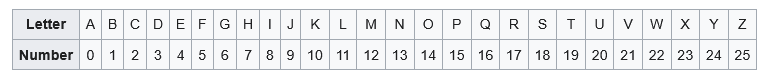
\includegraphics[width=0.85\textwidth]{../../images/python/page_009_img_01.png}

\end{document}
